\documentclass[10pt]{article}
\usepackage[margin=0.78in]{geometry}
\usepackage{amsmath,amssymb,bm,booktabs,graphicx,subcaption,url,microtype,float}
\captionsetup{font=small,skip=3pt}
\setlength{\textfloatsep}{6pt plus 2pt minus 2pt}
\setlength{\floatsep}{6pt plus 2pt minus 2pt}
\setlength{\intextsep}{6pt plus 2pt minus 2pt}
\graphicspath{{assets/figures/}}
\title{Supplementary Material: History-Aware Control Barrier Functions with Nonsingular Fading-Memory Kernels}
\author{Ege C. Altunkaya, Esra Demir, and \.{I}brahim \"Ozkol}
\date{}
\begin{document}
\maketitle
\section{Purpose and scope}
This companion collects the extended numerical material referenced by the six-page manuscript. Its role is to document the broader validation evidence and to show that the same history-conditioned authority mechanism persists beyond the one-state Caputo--Fabrizio (CF) realization used in the main paper.

The supplementary content is intentionally limited to three items: (i) the complete high-demand stress-test atlas, (ii) the bi-exponential-kernel benchmark, and (iii) the Gaussian-kernel benchmark.

\section{High-demand stress-test validation}
The high-demand validation sweep contains all $4\times 3\times 3=36$ combinations of square command level, release duration, and prepared history. Controller parameters are fixed across the sweep. Over all 36 cases, CF-FOCBF remains hard-safe, policy-safe, and feasible, while also reducing tracking RMSE relative to the history-blind policy-preserving CBF in every case.
\begin{figure}[H]
\centering
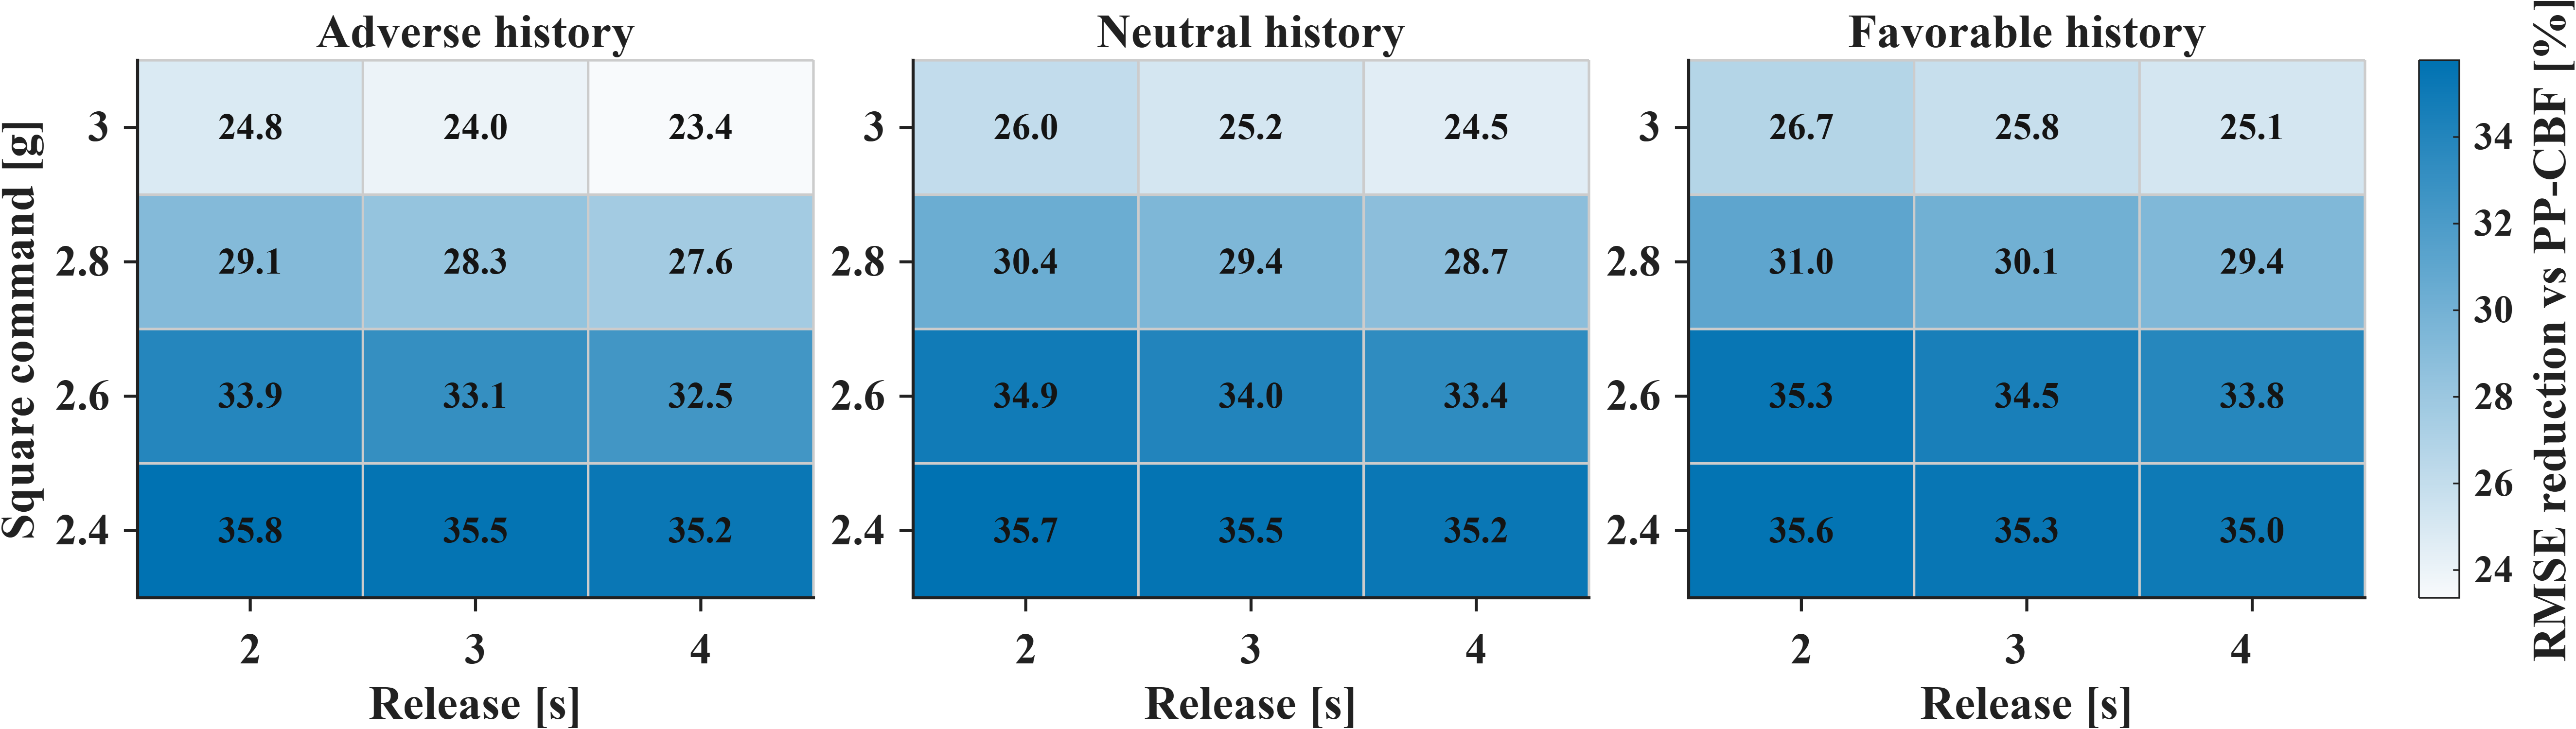
\includegraphics[width=0.97\textwidth]{stress_rmse_atlas.png}
\caption{Complete high-demand RMSE-reduction atlas. Each cell reports the percentage reduction of CF-FOCBF relative to the history-blind policy-preserving CBF for the same command, release duration, and prepared history.}
\end{figure}

\section{Beyond CF: kernel definitions}
For a generic nonsingular fading-memory kernel, the retained-history coordinate is
\begin{equation}
q_{\kappa}(t)=\int_{t_0}^{t}\kappa(t-\tau)\,\dot h(\tau)\,d\tau.
\end{equation}
The supplementary study compares the following three kernels.
\begin{align}
\kappa_{\mathrm{CF}}(s) &= \kappa_0 e^{-\lambda s},\\
\kappa_{\mathrm{BE}}(s) &= \kappa_0\left[a e^{-\lambda_1 s} + (1-a)e^{-\lambda_2 s}\right],\\
\kappa_{\mathrm{G}}(s)  &= \kappa_0 \exp\!\left[-\left(\frac{s}{\tau_G}\right)^2\right].
\end{align}
The CF kernel admits the exact one-state realization
\begin{equation}
\dot q=-\lambda q+\kappa_0\dot h.
\end{equation}
The bi-exponential kernel admits the exact two-state realization
\begin{equation}
\dot q_i=-\lambda_i q_i+\kappa_0\dot h,\qquad q=a q_1+(1-a)q_2.
\end{equation}
The Gaussian kernel is evaluated directly from retained history through the convolution integral itself, without replacing it by a finite-dimensional exponential surrogate.

\clearpage
\section{Bi-exponential kernel benchmark}
The same preparation protocol, common activation-state comparison, and twin-square maneuver are reused with the bi-exponential kernel. The adverse $<$ neutral $<$ favorable ordering is preserved both in the retained-history response and in the same-state admissible-control volume.
\begin{figure}[H]
\centering
\begin{subfigure}[t]{0.88\textwidth}
\centering
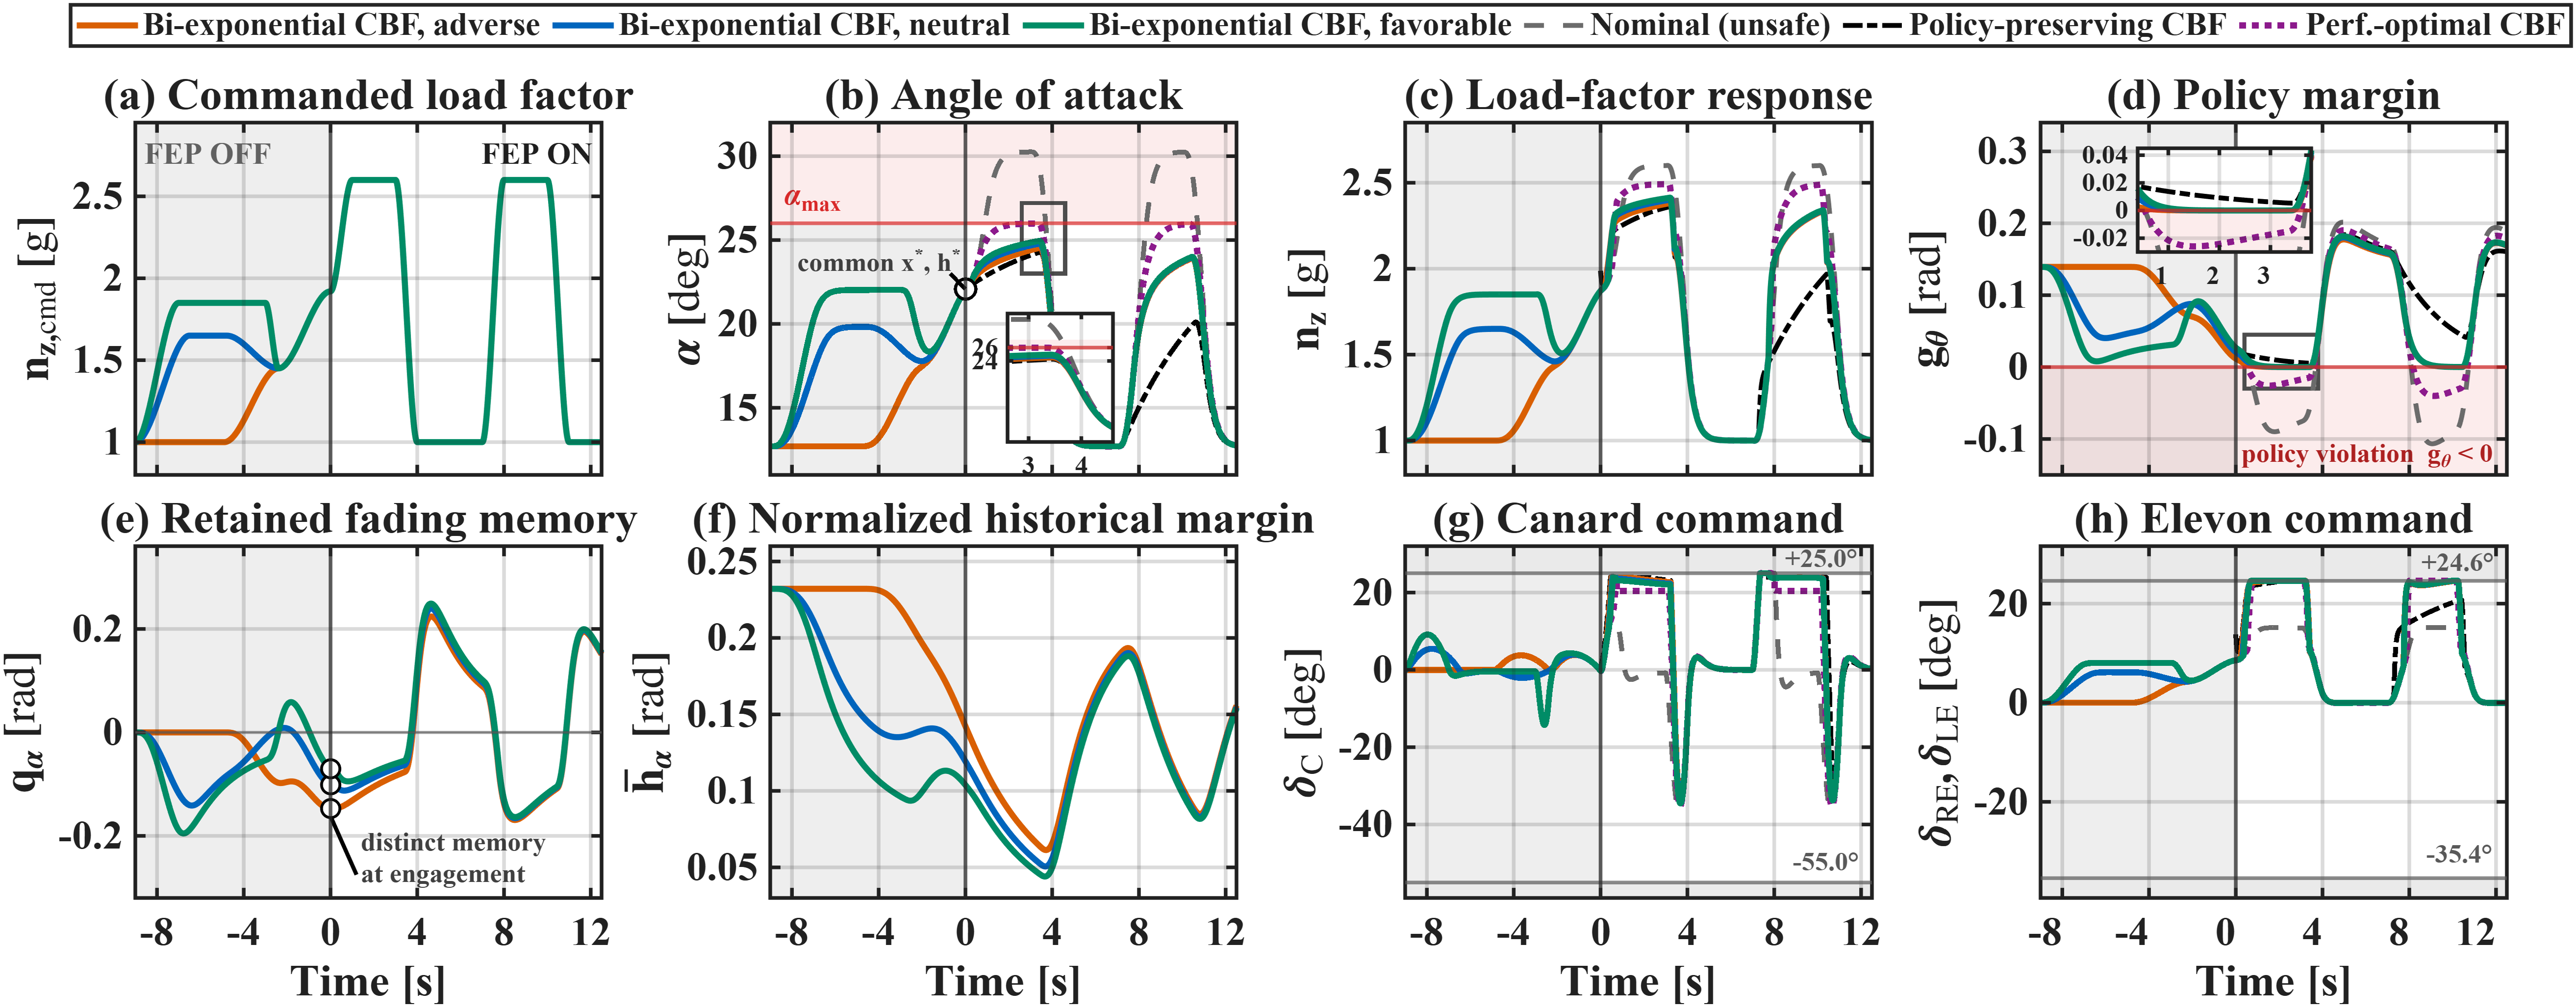
\includegraphics[width=\textwidth]{biexponential_stateResponse.png}
\caption{Twin-square benchmark under the bi-exponential kernel.}
\end{subfigure}
\vspace{0.25em}
\begin{subfigure}[t]{0.58\textwidth}
\centering
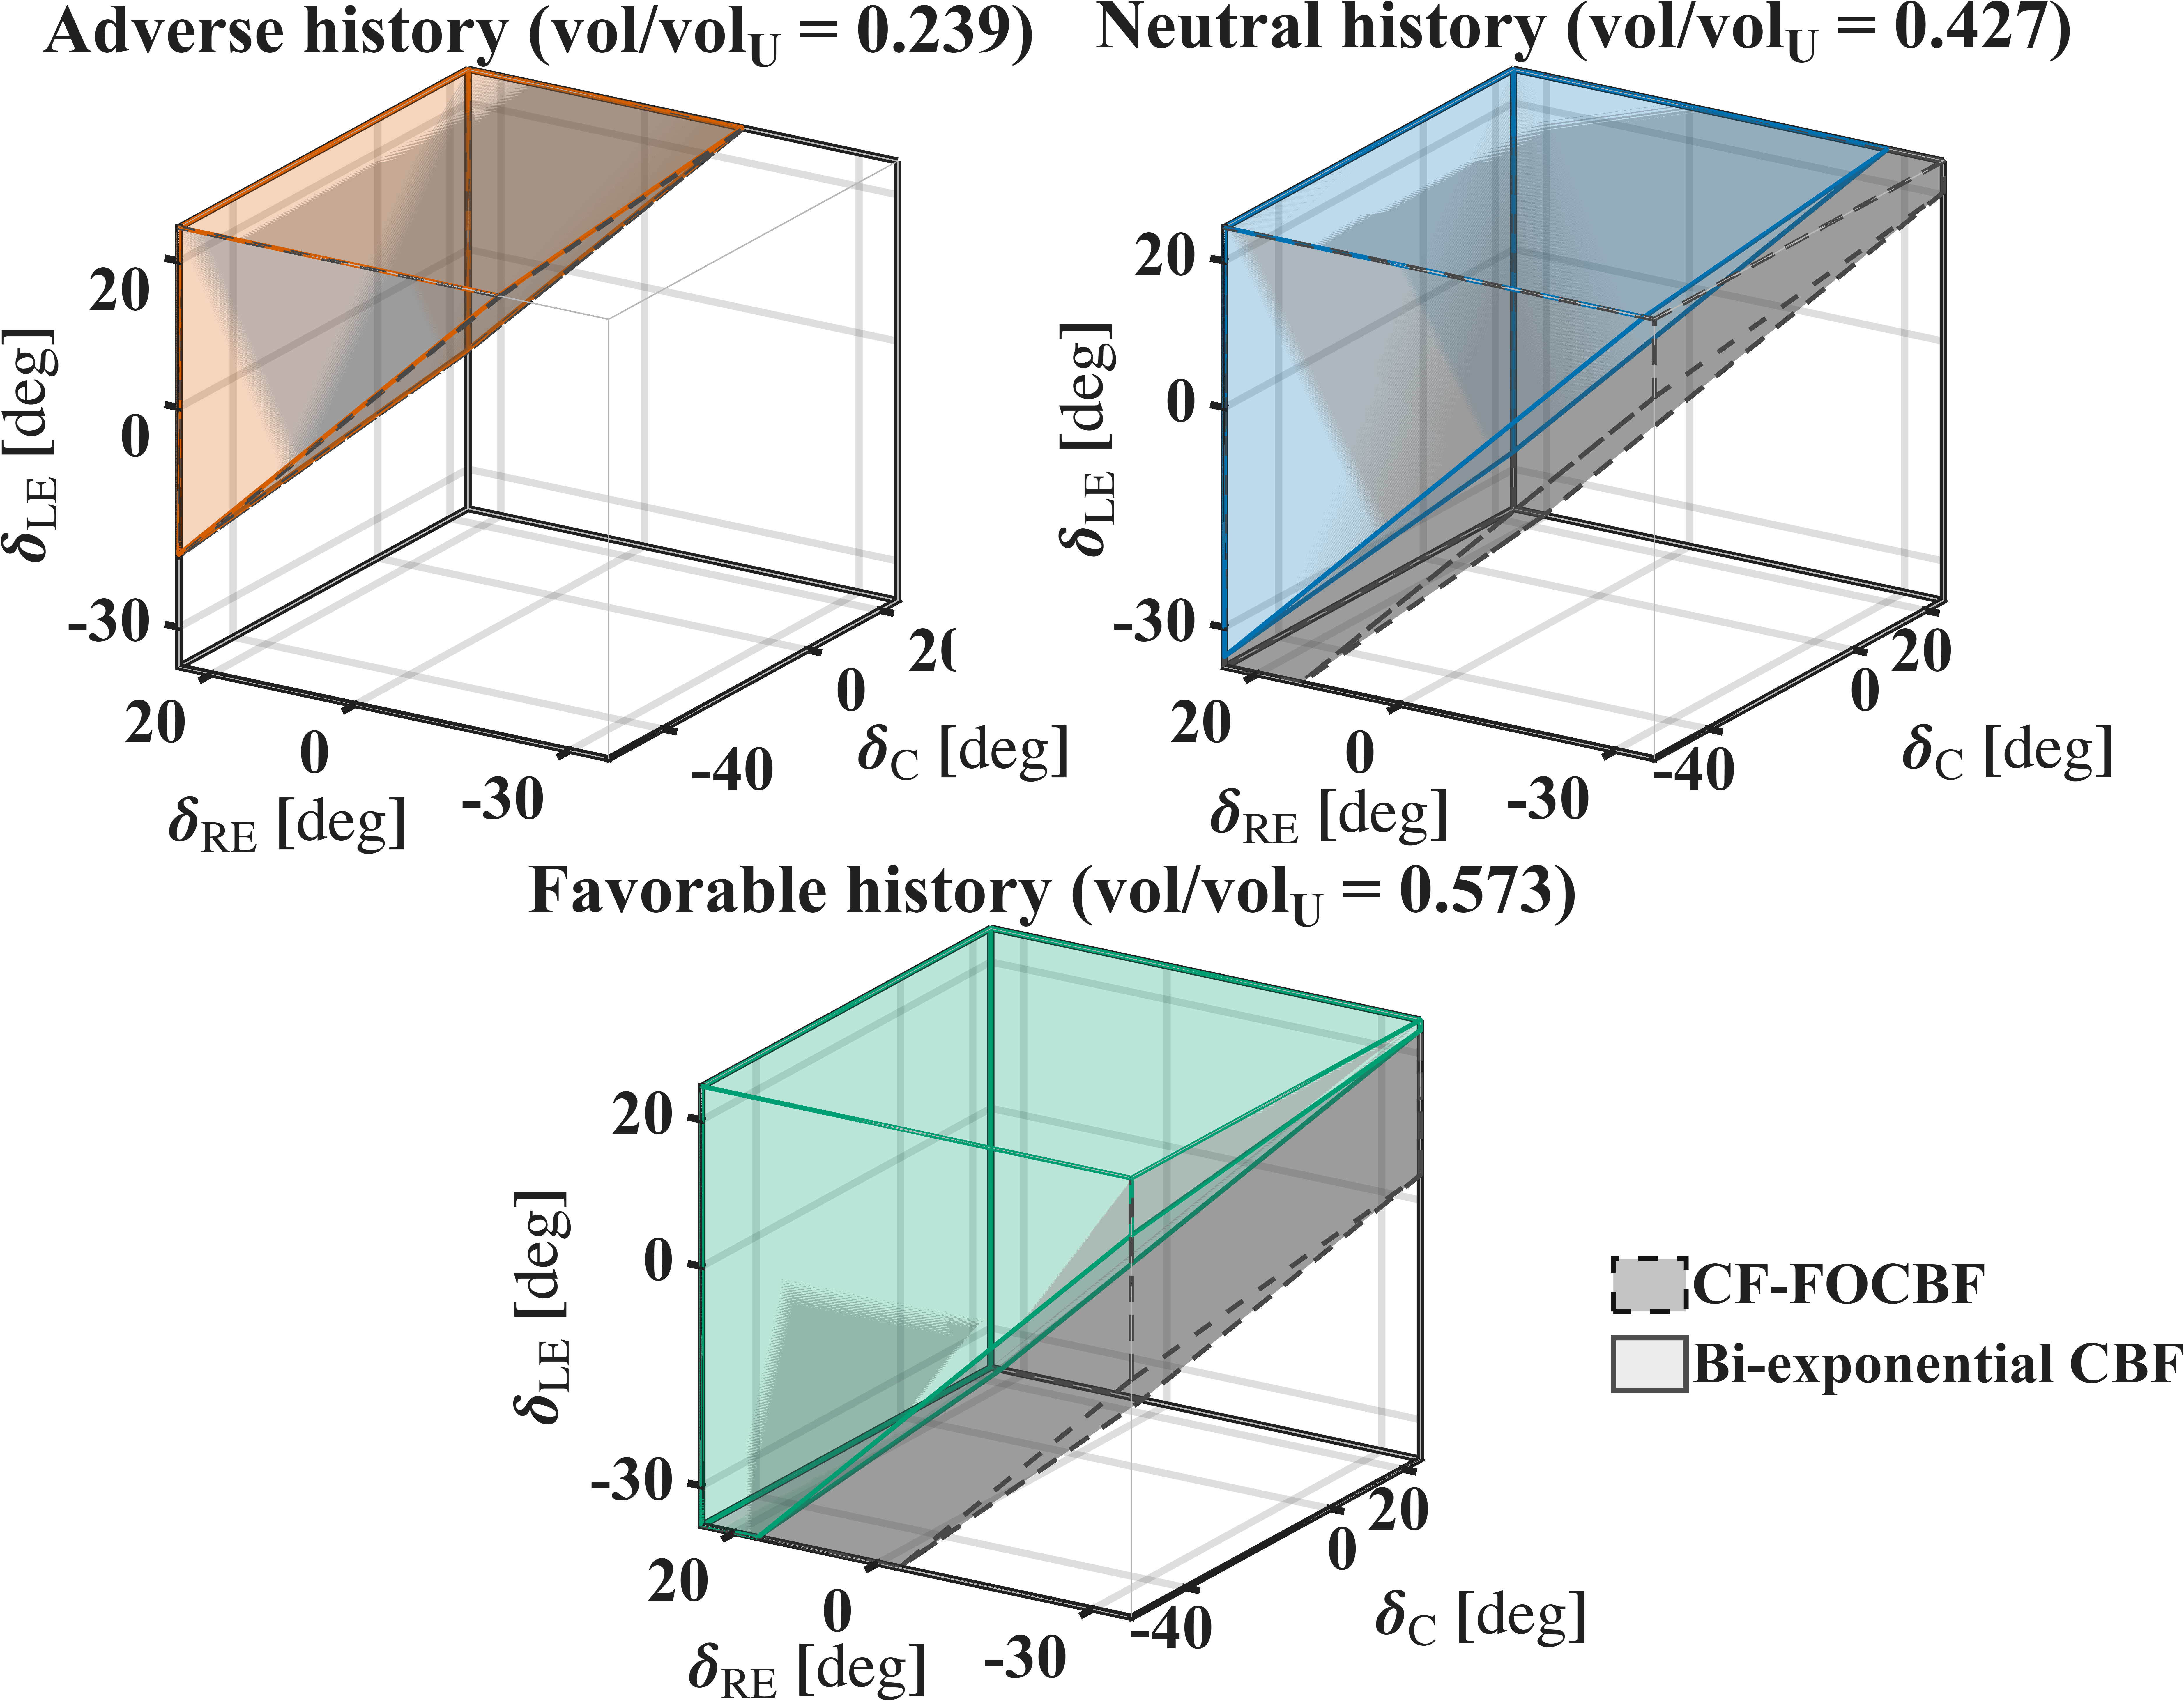
\includegraphics[width=\textwidth]{biexponential_admissibleSets.png}
\caption{Same-state admissible-set comparison under the bi-exponential kernel.}
\end{subfigure}
\caption{Bi-exponential-kernel validation. The mechanism remains visible with an exact two-state fading-memory realization.}
\end{figure}

\clearpage
\section{Gaussian kernel benchmark}
The Gaussian benchmark removes reliance on an exact finite-dimensional exponential realization and evaluates the memory term directly from retained history. The history-conditioned ordering again persists, demonstrating that the effect is not tied to the one-state CF implementation.
\begin{figure}[H]
\centering
\begin{subfigure}[t]{0.88\textwidth}
\centering

\includegraphics[width=\textwidth]{gaussian_stateResponse.png}
\caption{Twin-square benchmark under the Gaussian kernel.}
\end{subfigure}
\vspace{0.25em}
\begin{subfigure}[t]{0.58\textwidth}
\centering

\includegraphics[width=\textwidth]{gaussian_admissibleSets.png}
\caption{Same-state admissible-set comparison under the Gaussian kernel.}
\end{subfigure}
\caption{Gaussian-kernel validation. The retained-history mechanism remains visible even when the kernel is evaluated directly in the history domain.}
\end{figure}

\section{Availability}
The public GitHub Pages site collects the figures used in the manuscript companion. A cleaned and documented MATLAB package is being prepared for public release. Numerical datasets underlying the reported figures and tables are available from the corresponding author upon reasonable request.
\end{document}
